\subsection{График ФСЧ}
        
    Функцию стохастический чувствительности можно изобразить еще одним способом, который наглядно представлен на рисунках \ref{SSF_max} и \ref{SSF_min}.

    \begin{figure}
        \centering
        \subfloat[Максимум]{
            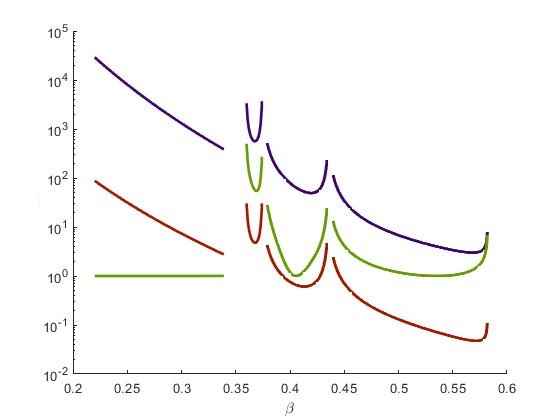
\includegraphics[width=0.9\textwidth]{stochastic/images/SSF_max.jpg}
            \label{SSF_max}
        }  
        
        \subfloat[Минимум]{
            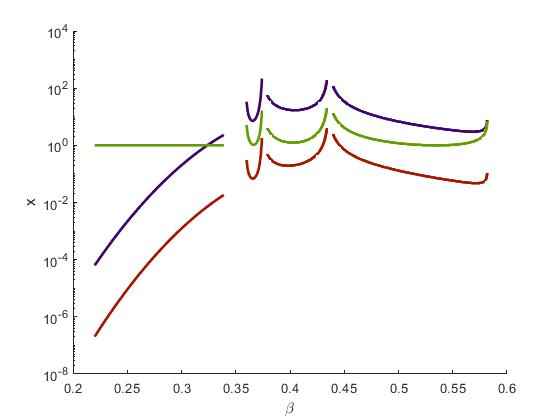
\includegraphics[width=0.9\textwidth]{stochastic/images/SSF_min.jpg}
            \label{SSF_min}
        }
            
        \caption{График функции стохастической чувствительности}
    \end{figure}
